%% abtex2-modelo-artigo.tex, v-1.9.5 laurocesar
%% Copyright 2012-2015 by abnTeX2 group at http://www.abntex.net.br/ 
%%
%% This work may be distributed and/or modified under the
%% conditions of the LaTeX Project Public License, either version 1.3
%% of this license or (at your option) any later version.
%% The latest version of this license is in
%%   http://www.latex-project.org/lppl.txt
%% and version 1.3 or later is part of all distributions of LaTeX
%% version 2005/12/01 or later.
%%
%% This work has the LPPL maintenance status `maintained'.
%% 
%% The Current Maintainer of this work is the abnTeX2 team, led
%% by Lauro César Araujo. Further information are available on 
%% http://www.abntex.net.br/
%%
%% This work consists of the files abntex2-modelo-artigo.tex and
%% abntex2-modelo-references.bib
%%

% ------------------------------------------------------------------------
% ------------------------------------------------------------------------
% abnTeX2: Modelo de Artigo Acadêmico em conformidade com
% ABNT NBR 6022:2003: Informação e documentação - Artigo em publicação 
% periódica científica impressa - Apresentação
% ------------------------------------------------------------------------
% ------------------------------------------------------------------------

\documentclass[
	% -- opções da classe memoir --
	article,			% indica que é um artigo acadêmico
	11pt,				% tamanho da fonte
	oneside,			% para impressão apenas no verso. Oposto a twoside
	a4paper,			% tamanho do papel. 
	% -- opções da classe abntex2 --
	%chapter=TITLE,		% títulos de capítulos convertidos em letras maiúsculas
	%section=TITLE,		% títulos de seções convertidos em letras maiúsculas
	%subsection=TITLE,	% títulos de subseções convertidos em letras maiúsculas
	%subsubsection=TITLE % títulos de subsubseções convertidos em letras maiúsculas
	% -- opções do pacote babel --
	english,			% idioma adicional para hifenização
	brazil,				% o último idioma é o principal do documento
	sumario=tradicional
	]{abntex2}


% ---
% PACOTES
% ---

% ---
% Pacotes fundamentais 
% ---
\usepackage{lmodern}			% Usa a fonte Latin Modern
\usepackage[T1]{fontenc}		% Selecao de codigos de fonte.
\usepackage[utf8]{inputenc}		% Codificacao do documento (conversão automática dos acentos)
\usepackage{indentfirst}		% Indenta o primeiro parágrafo de cada seção.
\usepackage{nomencl} 			% Lista de simbolos
\usepackage{color}				% Controle das cores
\usepackage{graphicx}			% Inclusão de gráficos
\usepackage{microtype} 			% para melhorias de justificação
% ---
		
% ---
% Pacotes adicionais, usados apenas no âmbito do Modelo Canônico do abnteX2
% ---
\usepackage{lipsum}				% para geração de dummy text
% ---
		
% ---
% Pacotes de citações
% ---
\usepackage[brazilian,hyperpageref]{backref}	 % Paginas com as citações na bibl
\usepackage[alf]{abntex2cite}	% Citações padrão ABNT
% ---

% ---
% Configurações do pacote backref
% Usado sem a opção hyperpageref de backref
\renewcommand{\backrefpagesname}{Citado na(s) página(s):~}
% Texto padrão antes do número das páginas
\renewcommand{\backref}{}
% Define os textos da citação
\renewcommand*{\backrefalt}[4]{
	\ifcase #1 %
		Nenhuma citação no texto.%
	\or
		Citado na página #2.%
	\else
		Citado #1 vezes nas páginas #2.%
	\fi}%
% ---

% ---
% Informações de dados para CAPA e FOLHA DE ROSTO
% ---
\titulo{Solução de Problemas de Valor no Contorno Bidimensionais}
\autor{Fernando Barbosa Neto \and Jeferson de Oliveira Batista}
\local{Vitória, Brasil}
\data{2015}
% ---

% ---
% Configurações de aparência do PDF final

% alterando o aspecto da cor azul
\definecolor{blue}{RGB}{41,5,195}

% informações do PDF
\makeatletter
\hypersetup{
     	%pagebackref=true,
		pdftitle={\@title}, 
		pdfauthor={\@author},
    	pdfsubject={Solução de Problemas de Valor no Contorno Bidimensionais},
	    pdfcreator={Fernando},
		pdfkeywords={valor de contorno}{bidimensionais}{solução}{problemas}{matriz esparsa}, 
		colorlinks=true,       		% false: boxed links; true: colored links
    	linkcolor=blue,          	% color of internal links
    	citecolor=blue,        		% color of links to bibliography
    	filecolor=magenta,      		% color of file links
		urlcolor=blue,
		bookmarksdepth=4
}
\makeatother
% --- 

% ---
% compila o indice
% ---
\makeindex
% ---

% ---
% Altera as margens padrões
% ---
\setlrmarginsandblock{3cm}{3cm}{*}
\setulmarginsandblock{3cm}{3cm}{*}
\checkandfixthelayout
% ---

% --- 
% Espaçamentos entre linhas e parágrafos 
% --- 

% O tamanho do parágrafo é dado por:
\setlength{\parindent}{1.3cm}

% Controle do espaçamento entre um parágrafo e outro:
\setlength{\parskip}{0.2cm}  % tente também \onelineskip

% Espaçamento simples
\SingleSpacing

% ----
% Início do documento
% ----
\begin{document}

% Seleciona o idioma do documento (conforme pacotes do babel)
%\selectlanguage{english}
\selectlanguage{brazil}

% Retira espaço extra obsoleto entre as frases.
\frenchspacing 

% ----------------------------------------------------------
% ELEMENTOS PRÉ-TEXTUAIS
% ----------------------------------------------------------

%---
%
% Se desejar escrever o artigo em duas colunas, descomente a linha abaixo
% e a linha com o texto ``FIM DE ARTIGO EM DUAS COLUNAS''.
% \twocolumn[    		% INICIO DE ARTIGO EM DUAS COLUNAS
%
%---
% página de titulo
\maketitle

% resumo em português
\begin{resumoumacoluna}
 Este relatório consiste nos detalhes da implementação em linguagem C e MatLab do programa de solução de problemas de valor no contorno bidimensionais com uso dos algoritmos eliminação de Gauss e do algoritmo SOR, ambos utilizando técnicas de armazenamento de matrizes esparsas, durante o processo de discretização pelo método das diferenças finitas. 
 
 \vspace{\onelineskip}
 
 \noindent
 \textbf{Palavras-chave}: equações diferenciais. sistemas lineares. valor no contorno. diferenças finitas. discretização.
\end{resumoumacoluna}

% ]  				% FIM DE ARTIGO EM DUAS COLUNAS
% ---

% ----------------------------------------------------------
% ELEMENTOS TEXTUAIS
% ----------------------------------------------------------
\textual

% ----------------------------------------------------------
% Introdução
% ----------------------------------------------------------
\section*{Introdução}
\addcontentsline{toc}{section}{Introdução}

Equações diferenciais pariciais aparecem com frequência na solução de problemas de várias áreas do conhecimento. Entretanto nem sempre é fácil encontrar uma solução analítica para determinada equação, por isso um método numérico pode ser útil ou essencial. 

O objetivo deste trabalho é implementar, em linguagem C e MatLab, um programa que solucione problemas de valor no contorno bidimensionais que utilizam implementações do algoritmo de eliminação de Gauss e do algoritmo SOR, ambos utilizando técnicas de armazenamento de matrizes esparsas. Estar-se-á utilizando o processo de discretização pelo método das diferenças finitas de equações do tipo:

\[ -\left(\frac{\partial^2 u}{\partial x^2}+\frac{\partial^2 u}{\partial y^2}\right)+a\frac{\partial u}{\partial x}+b\frac{\partial u}{\partial x}+cu=f(x,y) \]

Este relatório explanará nas futuras seções, através do referencial teórico utilizado, a implementação e os experimentos numéricos empregados a fim de obter o melhor resultado, especialmente no quesito performance, dos algoritmos. 


% ----------------------------------------------------------
% Seção de explicações
% ----------------------------------------------------------
\section{Referencial Teórico}

Equações diferenciais parciais, como mencionado anteriormente, surgem frequentemente em vários campos do mundo científico. Uma bastante conhecida e que aparece em diversos problemas tais como condução de calor, campo de potencial eletrostático, escoamento rotacional de um fluido sem viscosidade, torção de uma barra prismática, etc, é a equação diferencial de Laplace:

\[ -\left(\frac{\partial^2 u}{\partial x^2}+\frac{\partial^2 u}{\partial y^2}\right) = 0 \]

Um caso mais genérico de equação diferencial de segunda ordem é:

\begin{center} \[ -\left(\frac{\partial^2 u}{\partial x^2}+\frac{\partial^2 u}{\partial y^2}\right)+a\frac{\partial u}{\partial x}+b\frac{\partial u}{\partial x}+cu=f(x,y) \] em um domínio $ \Omega $ \end{center}

Onde a, b, c e f(x,y) são conhecidas e que u(x,y) é conhecida no contorno de $\Omega$. Desejando obter a solução u(x,y) no interior de um domínio retangular de dimensões $(x_{0},x_{(N+1)})\times(y_{0},y_{(N+1)})$, sendo conhecida a solução no contorno do retângulo, conhecida como condições de Dirichlet, são utilizadas para isso o método de discretização pelo método das diferenças finitas em alguns casos. Este método transforma a grade $m \times n$ em uma matriz pentadiagonal (para casos bidimensionais como estes) e um vetor independente, resultando em um sistema linear. Livros como Equações Diferenciais Elementares e Problemas de Valores de Contorno de Boyce e Diprima oferecem mais detalhes quanto à resolução aos casos aqui tratados.

Os sistemas lineares gerados no processo de discretização podem ser considerado esparsos dependendo do tamanho da matriz e devem ser resolvidos de forma a resgatar os valores de u(x,y) desejados. As formas de resolução abordadas são a Eliminação de Gauss e SOR. A primeira é considerado um método direto que consiste no, ao tratar matricialmente o sistema linear, escalonamento e, em seguida, substituições sucessivas e possui complexidade O($n^3$). A segunda é denominado como um método iterativo que, com o auxílio de um parâmetro de relaxação que deve possuir valores em [0,2[, contribuindo para alcançar uma resposta mais rapidamente ou divergir do resultado esperado, são realizadas iterações até atingir um erro menor que o desejado e possui complexidade O($n^2$), para cada iteração. Essa base teórica engloba principalmente as aulas ministradas pelo Professor Leonardo Muniz de Lima da disciplina de Algoritmos Numéricos I no período 2015/2 na Universidade Federal do Espírito Santo entre 4 de Agosto de 2015 e 1\textsuperscript{o} de Setembro de 2015. Também pode ser utilizado como material de apoio o livro Algoritmos Numéricos - Frederico Ferreira Campos, LTC, 2002.

Referindo-se à técnica de manipulação da matriz oriunda do sistema linear esparso, há conhecidas formas de compactação como o \emph{Compressed Sparse Row} (CSR), \emph{Compressed Sparse Column} (CSC) ou \emph{Skyline}. A implementação nativa em MatLab (Octave) da técnica de manipulação CSC foi utilizada nos experimentos aqui relatados, porém, em linguagem C, não foi buscado nenhuma dessas soluções a fim de desenvolver uma técnica própria que vise a melhor perfomance para as matrizes e os métodos de resolução a serem trabalhados. Dessa forma, em primeira instância, o foco utilizado para a compactação é o agrupamento dos elementos pelas suas respectivas colunas, ignorando os elementos nulos. Entretanto, durante a confecção do algoritmo, percebeu-se que o agrupamento por colunas era eficiente para a eliminação Gaussiana, enquanto para o SOR o mais adequado é o agrupamento de linhas. A implementação em termos de programação será descrita em detalhes na seção sobre Implementação.

\section{Implementação}

Nas subseções a seguir detalhar-se-á as implementações com as linguagens de programação C e MatLab (Octave).

\subsection{Implementação em C}

Para a compilação do módulo em C deve-se estar utilizando o terminal no diretório correto, o qual possui os arquivos do respectivo módulo, e far-se-á uso do comando \emph{make all} no referido terminal. Após este comando, para executar o programa compilado deve-se inicializá-lo, ainda no terminal, com a execução do arquivo programa gerado na forma do comando \emph{./programa}.

As subsções a seguir detalharão cada componente da implementação na linguagem de programação deste tópico.

\subsubsection{Entrada de dados}

A entrada de dados ocorre no arquivo main.c, onde o usuário poderá seguir as opções oferecidas no menu que lhe serão apresentados durante a execução do programa. 

É dada ao usuário a opção de escolha para a leitura dos dados: através do teclado ou através de um arquivo de entrada. Conforme orientado no parágrafo imediatamente anterior, basta seguir as instruções dos menus para obter o resultado desejado.

\subsubsection{Armazenamento e compactação matricial}

O tipo abstrato de dado (TAD) desenvolvido para o armazenamento e compactação da matriz pode ser encontrada nos arquivos listas.c e listas.h. A ideia inicial é um vetor de ponteiros, onde cada ponteiro é responsável por apontar na memória uma lista. Essas listas são dinamicamente alocadas e representam, cada uma delas, as colunas matriciais, compostas apenas dos elementos diferentes de zero.

O vetor de ponteiros foi declarado como uma \emph{struct}, chamando-a de coluna e definindo seu tipo posteriormente como Coluna. Cada tipo Coluna possui um ponteiro que aponta para o primeiro elemento. Os elementos são constituídos de \emph{struct elemento}, também atribuída definição de Elemento. Cada Elemento possui um inteiro l, representando a linha em que o elemento se encontra na matriz original, uma variável \emph{double} v, esta possuindo o valor do elemento na matriz original, e ponteiros do tipo Elemento que apontam tanto para o elemento anterior como para o próximo. Logo a matriz é, resumidamente, armazenada em um vetor de listas duplamente encadeadas. Oberserve que o próximo elemento do último de uma lista possui valor \emph{NULL} definido em stdlib.h, assim como o anterior do primeiro elemento.

listas.c compreende três funções de manipulação e criação da TAD da matriz. Uma delas possui assinatura \emph{Coluna* cria\_matriz(int tam);} que tem por objetivo a inicialização da matriz, cujos ponteiros do tipo Elemento apontam para \emph{NULL}. Outra dessas funções é \emph{void adiciona\_elemento(int l, int c, double valor, Coluna *matriz, int tam);}, cujo fim é para adicionar elementos à matriz, mas observando que esta função é tanto utilizada no processo de criação da matriz quanto durante os passos de resolução da mesma. A outra função, isto é, \emph{void imprime\_matriz(Coluna* matriz, int tam);}, auxilia no processo de \emph{debug} ao imprimir a matriz e não possui finalidade prática na resolução dos sistemas lineares diretamente. Outro detalhe a ser notado é que o vetor independente é considerada como uma coluna da matriz, logo as listas 0 a n de Coluna* matriz é a própria matriz focada enquanto a (n+1)-ésima lista refere-se ao vetor de termos independentes.

Apesar do foco inicial ser a implementação de um vetor de ponteiros para as colunas matriciais, ao desenvolver o método SOR percebeu-se que era necessário uma tática mais eficiente para o mesmo. Portanto, ao analisar o algoritmo deste método, foi buscada a implementação de vetor para as linhas matriciais, porém utilizada somente para este método. Para fins práticos, ao invés de criar um novo tipo abstrato de dado, ao adicionar o elemento no vetor de linhas bastava trocar o número da linha pelo número da coluna ao utilizar a função adiciona\_elemento, a qual foi explicada anteriormente. Observe que o último ponteiro, isto é, na posição n-ésima, diferentemente das posições 0 a n-1, armazenam o vetor independente, assim como na implementação anterior.

\subsubsection{Tratamento das Condições de Contorno}

O tratamento das condições de contorno se dá no arquivo contorno.c e sua respectiva biblioteca contorno.h, a qual possui inclusão de bibliotecas auxiliares e assinaturas das funções de contorno.c.

A função principal deste módulo é a que cuja assinatura é \emph{void contorna(double a, double b, double c, double xmin, double xmax, double ymin, double ymax, int divx, int divy, int tam, double valores[]);}, onde a, b e c são constantes da equação diferencial representada na introdução deste relatório, xmin, xmax, ymin e ymax são os valores mínimos e máximos para as variáveis x e y, divx e divx são as quantidades de partições em relação às abscissas e ordenadas, respectivamente, enquanto tam é o tamanho da matriz e valores é o vetor que armazena as condições de contorno. Nesta função são realizados os passos para tratamento das condições de contorno, cujo resultado é enviado para o arquivo de texto intermidiate.txt, o qual será lido posteriormente para criação das matrizes com tratamento de esparsidade, a fim de resolver o sistema linear resultante.

\subsubsection{Eliminação de Gauss}

O módulo responsável pela solução do sistema linear através da eliminação gaussiana encontra-se nos arquivos gauss.c e gauss.h. Tal solução é obtida com o uso de uma única função, cuja assinatura é \emph{void resolve\_gauss(Coluna *matriz, int n);}, onde \emph{matriz} é a matriz armazenada e compactada e \emph{n} é a ordem da matriz original.

O algoritmo se assemelha, estruturalmente falando, a um algoritmo comum de eliminação de Gauss, porém adequada ao tipo de dados em que está sendo trabalhado. \emph{Elemento *atual[n+1]} representa a linha atual que irá escalonar as linhas posteriores, sendo estas controladas por \emph{Elemento *subatual[n+1]}, sendo que ambos ponteiros de índice n trabalham no vetor independente devido à estrutura do TAD criado. Para percorrer as colunas a fim de encontrar um elemento de determinadas linhas, são utilizados \emph{while}s para iterar entre os elementos a fim de identificar o elemento da linha desejada. Um detalhe incomum decorrente da implementação ocorre na seguinte situação: se a x-ésima linha está escalonando a y-ésima linha e o elemento da posição (a,x) é diferente de zero enquanto o da posição (a,y) é nulo, logo o elemento em (a,y) não estará na matriz compactada. Para resolver este impasse, é invocada a função adiciona\_elemento declarada em listas.c, criando um elemento com valor zero (0), prosseguindo em seguida no escalonamento da linha referida.

Após o escalonamento, é utilizado o algoritmo de substituição sucessivas, o qual é deveras semelhante a um algoritmo de substituição sucessivas comuns, porém adequado ao tipo de dado que se está trabalhando. A resposta é armazenada no vetor \emph{double resp[n]}, o qual será direcionado para a função saída\_de\_dados, declarada em saida.c, escrevendo a respostas no respectivo arquivo de saída.

O tempo é marcado logo antes do escalonamento na eliminação de Gauss e termina logo após as substituições através da função clock\_gettime da biblioteca time.h. Para mais informações sobre a marcação do tempo e resultados, ver seção 3 Experimentos Numéricos.

\subsubsection{SOR}

O módulo responsável pela solução do sistema linear através do método SOR encontra-se nos arquivos sor.c e sor.h.

Primeiramente, como adiantado nas seções e subseções anteriores,  foi utilizado como estratégia inicial a mesma do método de eliminação de Gauss: vetor de listas, as quais representam as colunas da matriz. O algoritmo conforme esta implementação pode ser encontrado na função de assinatura \emph{void resolve\_sor(Coluna *matriz, int n, double omega, double toler);}. Os parâmetros são matriz, que é a matriz oriunda do sistema linear, n, a ordem da matriz, omega, que é o parâmetro de relaxação, e toler, este a tolerância que determina o critério de parada consequente do erro normal utilizado. Todavia esta tática possuía uma perfomance decepcionante ao comparada com o método direto. Portanto, ao analisar o algoritmo, percebeu-se que seria mais prático e eficiente utilizar ainda um vetor de listas, porém agora estas representando as linhas da matriz. De qualquer forma, foi mantida essa função derivada de tal implementação no código para fins de curiosidade do leitor. 

Para a segunda implementação, foi criada a função \emph{void resolve\_sor2(Coluna *matriz, int n, double omega, double toler);}, cujos parâmetros possuem mesmo propósito explanados na implementação anterior. Ambas as implementações utilizam um algoritmo simples para o SOR, portanto apenas traduzido de um pseudocódigo para a linguagem C e, logicamente, com os devidos ajustes para os casos de matrizes esparsas e respectivas implementações. Uma ressalva ao comparar o algoritmo em C com um pseudocódigo é que foi utilizado o aproveitamento de variável, evitando que várias sejam declaradas para um breve fim. Lembre-se que esta agora é a correta implementação para este método.

Em ambas implementações do SOR foi utilizada para critério de parada, a fim de se comparar com a tolerência providenciada, a norma-$\infty$. Como não é definido um número máximo de iterações, pois isso exigiria mais processamento para verificação de mais um critério de parada, é necessário verificar manualmente, por exemplo, inserindo \emph{printf} para ser analisada a variação dos erros em tempo de execução.

O tempo é calculado a partir do início do algoritmo de fato e a contagem é terminada logo após o erro normal ser menor que a tolerância. Para este objetivo, foi utilizada a função clock\_gettime da biblioteca time.h. Para mais informações sobre a marcação do tempo e resultados, ver seção 3 Experimentos Numéricos.

\subsubsection{Saída de dados}

A saída dos dados compreende os módulos saida.c e saida.h. É o módulo mais simples e possui apenas a função de assinatura \emph{void saida\_de\_dados(int n, double resp[]);}, a qual recebe como parâmetros uma variável do tipo inteiro que representa a quantidade de elementos do segundo parâmetro, o qual é um vetor de \emph{double} que armazena as respostas do método utilizado. Os resultados contidos nesse vetor são escritos no arquivo de saída cujo nome é determinado pelo usuário. Observe que a primeira linha deste arquivo indica o tamanho do vetor-resposta, enquanto as demais linhas corresponde à solução propriamente dita, da variável x(0) até x(n-1).

Também é possível imprimir alternativamente o resultado na tela, desde que selecionada esta opção, vide menu de opções de saída do programa.

\subsection{Implementação em MatLab (Octave)}

A utilização das funções em MatLab (Octave) para a resolução dos Problemas do Valor de Contorno deve se dar no diretório que contém os arquivos
das referidas funções, sendo que há uma função, a \emph{main} responsável por toda a interface com o usuário e pela utilização
das demais funções para solução do problema.

\subsubsection{Entrada de dados}

Durante a execução da função \emph{main} será apresentado duas opções para entrada dos dados ao usuário, sendo uma por teclado
e outra por arquivo de entrada. A própria \emph{main} fornecerá informações relativas aos dados e ao formato dos mesmos, caso a
entrada por teclado seja escolhida. Sendo assim, o usuário precisa apenas seguir as instruções dadas para alcançar o resultado desejado.

Caso a entrada por arquivo seja a opção do usuário, o programa pedirá ao usuário que digite o nome do arquivo de entrada. Tal arquivo
deve conter os dados do problema no seguinte formato e ordem:

A primeira linha deve conter os coeficientes a, b, c, separados por espaços.

A segunda linha informa a grade do domínio do problema no seguinte formato:
\begin{center} \emph{xmin xmax ymin ymax n m} \end{center}
Onde \emph{n} é o número de pontos na abscissa e \emph{m} é o números de pontos na ordenada.

A terceira linha possui apenas um número inteiro, que informa a \emph{f(x,y)} da equação diferencial, sendo:
\begin{flushleft} 
1 - Para $ f(x,y) = 0 $ \newline
2 - Para $ f(x,y) $ tal que $ u(x,y) = x e^{xy} sen(\pi x) cos(\pi y) $ 
\end{flushleft}

A quarta linha possui um inteiro informando o formato no qual serão inseridos os valores de contorno, sendo:
\begin{flushleft}
1 - Para inserção de todos os valores de contorno \newline
2 - Para um valor constante em todo o contorno \newline
3 - Para aplicação da $ u(x,y) = x e^{xy} sen(\pi x) cos(\pi y) $ em todo o contorno
\end{flushleft}

A quinta linha informará os valores de contorno, de acordo com o formato indicado na quarta linha. Caso a opção selecionada
seja a primeira, todos os valores de contorno devem estar escritos, separados por espaços. Caso a opção seja a segunda, apenas
um valor é apresentado nessa linha. Se a opção for a terceira, a quinta linha ficará vazia.

A sexta linha apresenta um inteiro que informa qual método de resolução será utilizado, sendo:
\begin{flushleft}
1 - Para o método iterativo Succesive Over-Relaxation (SOR) \newline
2 - Para o método exato de eliminação gaussiana
\end{flushleft}

A sétima linha informa, também através de um inteiro, onde deve ser apresentada a saída, sendo:
\begin{flushleft}
1 - Para impressão da solução na tela \newline
2 - Para escrita da solução no arquivo saida.txt
\end{flushleft}

Caso o usuário opte pelo SOR, haverá ainda uma oitava linha, informando os parâmetros \emph{tol}, que é a tolerância máxima
desejada; \emph{kmax}, que é o número máximo de iterações; e \emph{w}, que é o fator de relaxação.

\subsubsection{Armazenamento e compactação matricial}

A estrutura utilizada para o armazenamento da matriz esparsa presente no sistema linear que soluciona o Problema de Valor de Contorno
é a estrutura presente no próprio Octave chamada Compressed Column Sparse, ou CCS, onde apenas os elementos não-nulos são armazenados.

O uso da estrutura CCS ocorre na função \emph{montarMatriz(a, b, c, grade)} com a chamada de \emph{sparse(N, N)} onde \emph{N} é a ordem da matriz.

Na referida função \emph{a, b, c} são os coefientes da equação diferencial, enquanto que grade é um vetor contendo os seguintes valores:
\emph{xmin} que é o menor valor de abscissa na grade do domínio; \emph{xmax} que é o maior valor de abscissa; \emph{ymin} que é
o menor valor de ordenada; \emph{ymax} que é o maior valor de ordenada; \emph{n} que é o número de valores na abscissa; e \emph{m}
que é o número de valores na ordenada. O retorno dessa função é uma matriz esparsa \emph{M} e um vetor \emph{coef} que é útil
no tratamento das condições de contorno.

\subsubsection{Tratamento das Condições de Contorno}

O tratamento das condições de contorno se dá na função \emph{tratarContorno(v, valores, coef, n, m)} onde \emph{v} é o vetor independente
original do sistema, ou seja, sem o tratamento das condições de contorno; \emph{valores} é um vetor contendo a imagem de todos os pontos
no contorno da grade; \emph{coef} é um vetor fornecido pela função \emph{montarMatriz} que auxilia no tratamento, como dito anteriormente;
\emph{n} e \emph{m} têm o mesmo significado que no vetor \emph{grade}, representando as dimensões da grade do domínio.

A função \emph{tratarContorno} tem como retorno o mesmo vetor \emph{v} com as condições de contorno tratadas.

\subsubsection{Eliminação de Gauss}

Caso a função solicitada pelo usuário para a resolução do sistema linear resultante do Problema de Valor de Contorno seja o método exato, que é a eliminação de Gauss, a própria função \emph{built-in} presente em Octave, representada por $\backslash$, é então chamada.
Como entrada, essa função recebe a matriz resultante da função \emph{montarMatriz} e o vetor resultante da função \emph{vetorIndependente}
depois de tratado por \emph{tratarContorno}.

A função retorna a solução numérica do problema em todos os pontos no interior da grade do domínio.

\subsubsection{SOR}

Caso a função solicitada pelo usuário seja o método iterativo SOR, é chamada então a função \emph{sor(A, b, n, tol, kmax, w)},
presente em \emph{sor.m}, onde \emph{A} recebe a matriz esparsa resultante de \emph{montarMatriz}; \emph{b} recebe o vetor resultante de \emph{vetorIndependente}
depois de tratado por \emph{tratarContorno}; \emph{n} recebe a ordem do sistema linear; \emph{tol} é o erro máximo tolerado;
\emph{kmax} é o número máximo de iterações; e \emph{w} é o fator de relaxação.

A função retorna o vetor \emph{[x, iter, erro, tempo]}, onde \emph{x} é o vetor solução; \emph{iter} o número de iterações gastas;
\emph{erro} a estimativa do erro cometido; e \emph{tempo} o tempo gasto na execução da função \emph{sor}.

\subsubsection{Saída de dados}

A solução do sistema linear resultante do Problema de Valor de Contorno e calculada por um dos métodos de solução, pode ser
impressa na tela ou escrita em um arquivo saida.txt, de acordo com a preferência do usuário, como está relatado na seção 2.2.1.

\section{Experimentos Numéricos}

A seguir serão apresentados os resultados e observações dos experimentos numéricos para ambas as implementações.

\subsection{Implementação em C}

Primeiramente, para verificar que o resultado da implementação retorna respostas coerentes, pode ser utilizado o arquivo funciona.txt. Neste arquivo há os parâmetros para a equação de Laplace com x variando de 0,0 a 12,8 e y variando de 0,0 a 8,0, além de 6 e 5 divisões nas abscissas e ordenadas da grade, respectivamente. Neste caso foi utilizado contorno constante de 12, como pode ser verificado no mesmo arquivo. Ao compilar o programa com \emph{make all} e executá-lo em seguida como \emph{./programa}, seleciona-se a opção do algoritmo desejado, no próximo menu escolha a opção 2 e em seguida entre com funciona.txt, escolhendo logo após o modo de saída para comparar o resultado. Como esperado, a resposta deverá ser 12 para todo ponto u(x,y). No caso do SOR para o arquivo funciona.txt recomenda-se usar 0.00001 como tolerância e 1.5 de fator de relaxação.

Para medição e comparação dos tempos de processamento da construçao do sistema linear e dos algoritmos de Eliminação de Gauss e SOR, foram utilizados os recursos providos da biblioteca de C chamada time.h, enviando mensagens para stdout com os tempos logo antes de pedir a opção de saída. As características em questão de hardware e software do equipamento utilizado para medição temporal é: Notebook Dell Vostro 3460, com Sistema Operacional Ubuntu 15.04 64-bit, memória de 5.7 GiB, processador Intel® Core™ i5-3230M CPU @ 2.60GHz x 4 e placa de vídeo GeForce GT 630M/PCIe/SSE2. 

Os tempos de processamento estão sumarizados na Tabela 1 a seguir. Observe que os tempos estão em segundos e que C X refere-se ao tempo de construção do sistema linear com algoritmo X, R X é a resolução desse sistema com algoritmo X e T X é a soma do tempo de construção com o de resolução. Também estão especificados os tamanhos das malhas trabalhadas. A equação foi utilizada em $\Omega$ = $\{(x,y) : 0 \leq x,y \leq 1\}$ com a = 60, b = 80, c = -40 e f(x,y) é tal que $u(x,y)=x e^{xy} \sin (\pi x) \cos (\pi y)$. Os arquivos de entrada para o caso de ordem K pode ser encontrado em K.txt, exemplo: o caso 8x8 está localizado no arquivo 8.txt. Estes casos de teste foram gerados com o programa auxiliar provido por gerador.c. A tolerância usada nos testes do SOR é de $10^{-5}$.

\begin{table}[!h]
\centering
\caption{Tempos de processamento em C}
\label{my-label}
\begin{tabular}{|l|l|l|l|l|l|l|l|l|}
\hline
Malha   & C Gauss & R Gauss & T Gauss & C SOR & $\omega$ & Iterações & R SOR & T SOR \\ \hline
8x8     & 0.001266 & 0.000191 & 0.001457 & 0.000868 & 0.3 & 39 & 0.000165 & 0.001033 \\ \hline
16x16   & 0.003221 & 0.006839 & 0.010060 & 0.003032 & 0.6 & 23 & 0.000484 & 0.003516 \\ \hline
32x32   & 0.017964 & 0.175472 & 0.193436 & 0.018893 & 1.1 & 60 & 0.005772 & 0.024665 \\ \hline
64x64   & 0.102360 & 5.073515 & 5.175875 & 0.100288 & 1.5 & 56 & 0.014464 & 0.114752 \\ \hline
128x128 & 0.640980 & 273.145311 & 273.786291 & 0.624195 & 1.7 & 82 & 0.080149 & 0.704344 \\ \hline
256x256 & 8.392534 & 15713.142233 & 15721.53476 & 8.494499 & 1.8 & 101 & 0.299954 & 8.794453 \\ \hline
\end{tabular}
\end{table}

Algumas observações podem ser levantadas da Tabela 1, a começar pelo grande aumento no tempo de processamento no caso das construções do sistema linear e a resolução pelo algoritmo da eliminação Gaussiana. Isso ocorre pois, ao duplicar a ordem da grade, a matriz resultante do sistema linear fica aproximadamente 4 vezes maior em número de linhas e um algoritmo de complexidade O($n^3$) como o de Gauss causaria um acréscimo temporal teórico de 64 vezes. A taxa de crescimento de 64 para acréscimo nos tempos não é replicado pois as matrizes tem tratamento esparsial, decrescendo significativamente o tempo para obter a solução do sistema.

Quanto ao SOR, foram utilizados parâmetros de relaxação ($\omega$) que, na iminência da divergência, pudessem gerar o resultado mais rapidamente possível. Interessante notar que, devido à esparsidade aumentar juntamente com o aumento da ordem da malha, o $\omega$ pode aumentar junto com o aumento da matriz do sistema, oferecendo resultados relativamente muito bons em termos de desempenho.

\subsection{Implementação em MatLab}

Primeiramente, foram realizados experimentos relativos a equação de Laplace, utilizando um valor constante em todo o contorno
do domínio. Para isso, foi inserido como arquivo de entrada o eqLaplaceExato.txt, que possui dados de uma equação de Laplace, 
descreve um contorno com valor constante igual a  12.0 e faz chamada do método exato. Pelo arquivo saida.txt gerado por essa
entrada, percebe-se que a solução do sistema é constante e igual a 12.0 em todo o domínio. Foi gasto um tempo de $ 0.0051520 s $
na execução da função built-in $ \backslash $ do MatLab (Octave). [Há uma descrição do hardware utilizada, posteriormente,
nessa mesma seção]. Também foi inserido o arquivo eqLaplaceIterativo.txt para o resolução do mesmo problema, porém utilizando o método SOR. Obtivemos
um solução bem parecida (valores bem próximos de 12.0 em todo o domínio) e o tempo gasto na execução da função \emph{sor} foi
$ 75.525 s $ após 140 iterações.

A grade descrita em eqLaplaceExato.txt é uma 64x64, enquanto que a de eqLaplaceIterativo.txt é uma 16x16. Não se pode comparar
as funções $ \backslash $ e \emph{sor} diretamente, já que a primeira é built-in. Nesse experimento com o SOR foi utilizado uma
tolerância de 0.00001, número máximo de iterações igual a 5000 e um fator de relaxação de 1.5.

Para medição e comparação dos tempos de processamento dos algoritmos de Eliminação de Gauss e SOR, foram utilizadas duas funções
nativas do MatLab (Octave), a \emph{tic}, que inicia a contagem de tempo, e a \emph{toc}, que finaliza a contagem de tempo e retorna
o tempo gasto. As características em questão de hardware e software do equipamento utilizado para medição temporal é: 
Microcomputador Multilaser, com processador Intel® Core™ i5-2310 CPU @ 2.90GHz x 4,
placa de vídeo Gallium 0.4 on NVCF, memória de 194,6 GB, Sistema Operacional Ubuntu 15.10 64-bit.

Os tempos de processamento estão sumarizados na Tabela 2 a seguir. Observe que os tempos estão em segundos e que R X é o tempo gasto na resolução desse sistema com o algoritmo X. Também estão especificados os tamanhos das malhas trabalhadas. A equação foi utilizada em $\Omega$ = $\{(x,y) : 0 \leq x,y \leq 1\}$ com a = 60, b = 80, c = -40 e f(x,y) é tal que $u(x,y)=x e^{xy} \sin (\pi x) \cos (\pi y)$. Os arquivos de entrada para o caso de ordem K podem ser encontrados em ``malha K eg'' (para método exato) e em ``malha K sor'' (método iterativo), exemplo: o caso 8x8 do método SOR está localizado no arquivo ``malha 8 sor''. A tolerância usada nos testes do SOR é de $10^{-5}$.

\begin{table}[!h]
\centering
\caption{Tempos de processamento em MatLab (Octave)}
\label{my-label}
\begin{tabular}{|l|l|l|l|l|}
\hline
Malha   & R Gauss & {w} & Iterações & R SOR \\ \hline
8x8     & 8.9312e-04 & 0.05 & 245 & 4.7859 \\ \hline
16x16   & 0.0014470 & 0.2 & 44 & 24.288  \\ \hline
32x32   & 0.0029218 & 0.8 & 12 & 147.25  \\ \hline
64x64   & 0.012709 & 1.6 & * & *  \\ \hline
128x128 & 0.076514 & 1.6 & * & * \\ \hline
256x256 & 0.28344 & 1.6 & * & * \\ \hline
\end{tabular}
\end{table}

* = Tempo limite de 1 hora de processamento contínuo atingido e, portante, teste abortado. Par ao caso de 64x64 é estimado 3,5 minutos para cada iteração do SOR.

É possível tirar algumas conclusões com base nos dados apresentados na tabela acima. Uma delas é que, pelo método exato ter 
complexidade $ O(n^3) $, de um caso para o próximo, deveríamos ter um tempo de resolução 64 vezes maior. Porém, o que ocorre na
prática é que, o tempo de processamento aumenta em uma taxa de 4 vezes, em média, na solução exata, devido ao tratamento da
esparsidade.

No caso do método SOR, de um caso para o próximo, ou seja, dobrando-se as dimensões da malha, observa-se pela tabela que o
aumento no tempo de processamento de uma iteração aumenta de acordo com a previsão teórica, ou seja, como cada iteração tem
complexidade $ O(n^2) $, temos uma taxa de cerca de 16 vezes do aumento do tempo de resolução. Dessa forma, concluímos que
o armazenamento da matriz do sistema linear utilizando a técnica CSC ocasionou menor consumo de memória, mas não melhor desempenho.
Temos duas hipóteses para isso. A primeira é que o método SOR, por sua própria natureza, não melhora o seu desempenho com o tratamento
da esparsidade. Outra é que pode ser que a implementação do SOR em alto nível não tire vantagens da matriz esparsa, em termos
de desempenho.

Como relatado em relação aos experimentos da implementação em C, quanto maior for a ordem da matriz do sistema linear, maior
é o fator de relaxação que podemos usar, sem que haja divergência no algoritmo SOR, pois o aumento da ordem da matriz acarreta
em aumento da esparsidade da mesma. Pode-se observar também, que o número de iterações necessárias diminui a medida que a ordem
da matriz aumenta, indicando que o algoritmo SOR converge mais rápido com fatores de relaxação maiores.

Os experimentos para as malhas 128x128 e 256x256, usando o método SOR não se apresentaram viáveis, já que, nesses casos, a estimativa
de tempo para uma iteração é maior que uma hora.
 
\subsubsection{Gráficos}

Para validar os experimentos quanto à sua corretude, o gráfico abaixo foi gerado pelo arquivo eqLaplaceExato.txt para solução da Equação de Laplace com contorno constante igual a 12. Pode-se perceber que o resultado condiz com o esperado: um plano na altura 12.

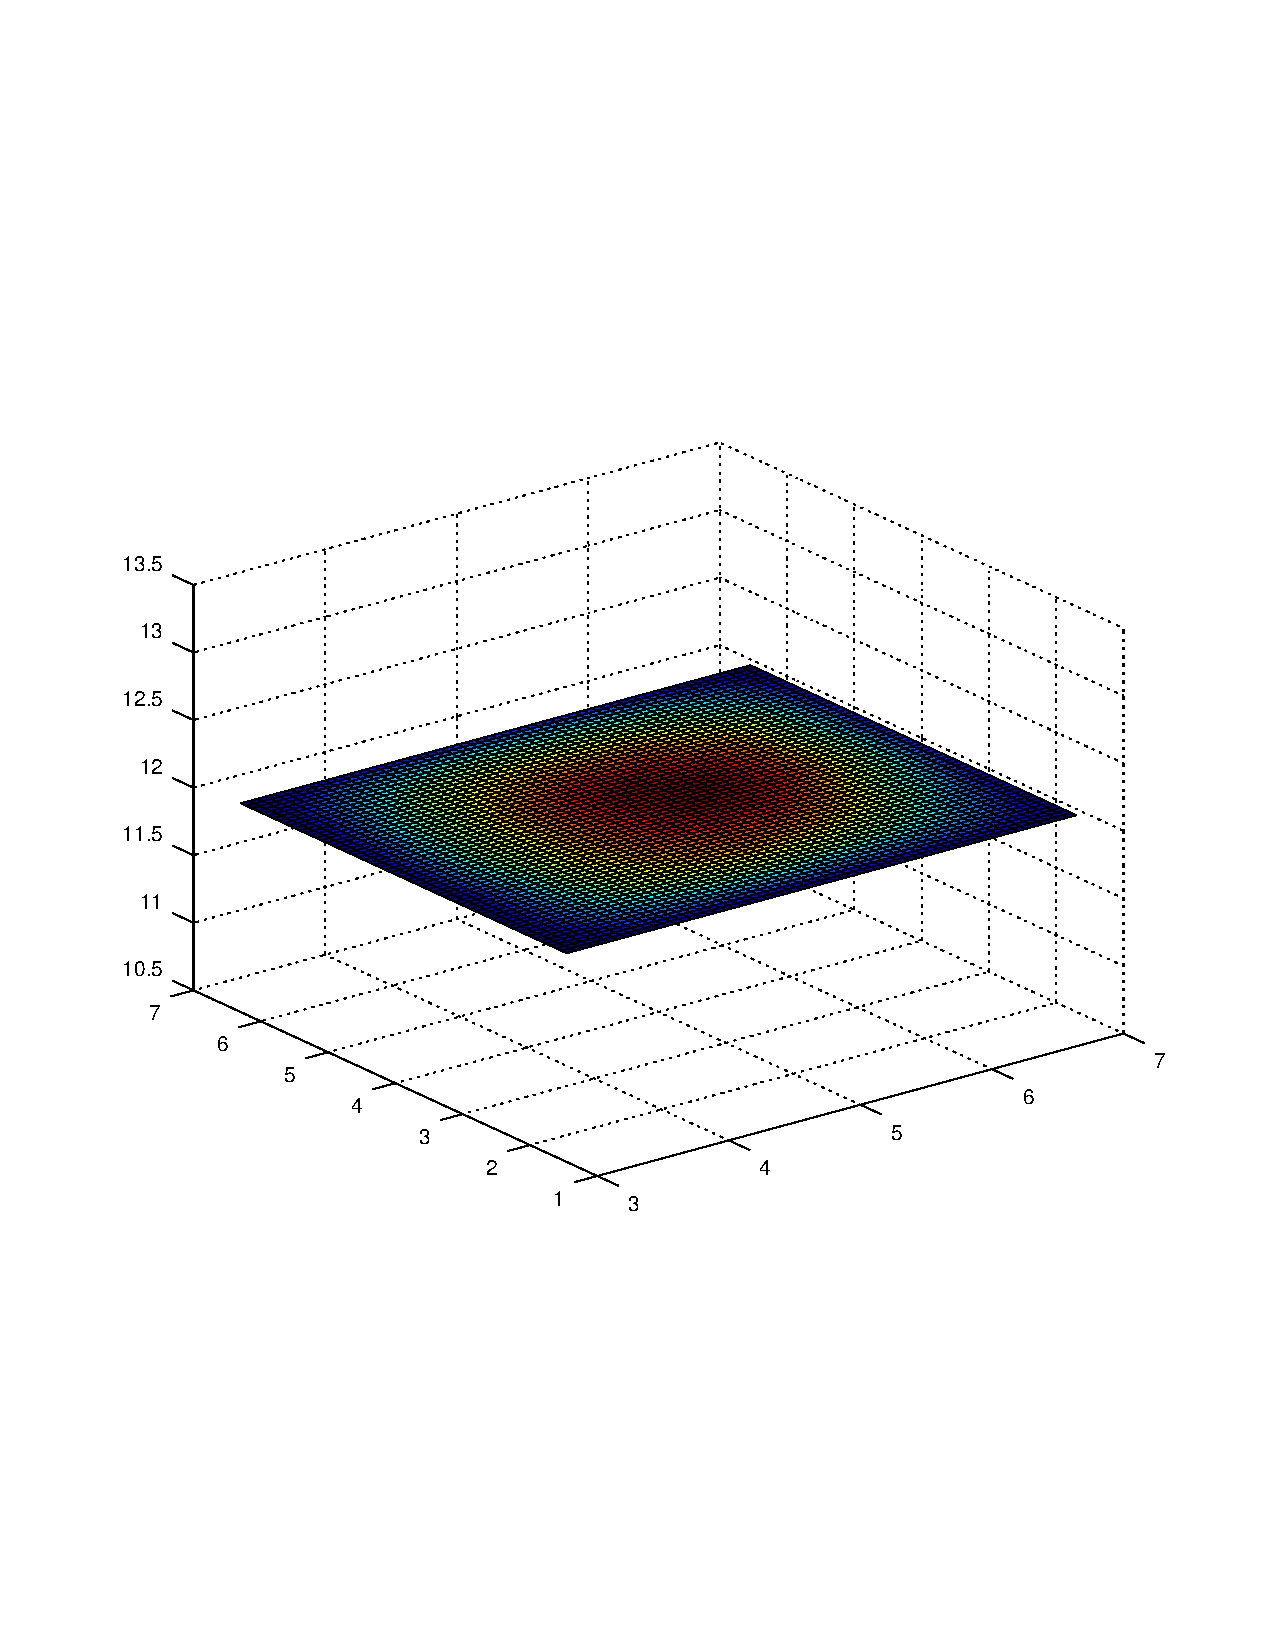
\includegraphics[scale=0.5]{eqLaplaceExato}

Abaixo também verifica-se a solução do arquivo "malha 128 eg", sem aspas, que representa a malha com contorno f(x,y) tal que $u(x,y)=x e^{xy} \sin (\pi x) \cos (\pi y)$.

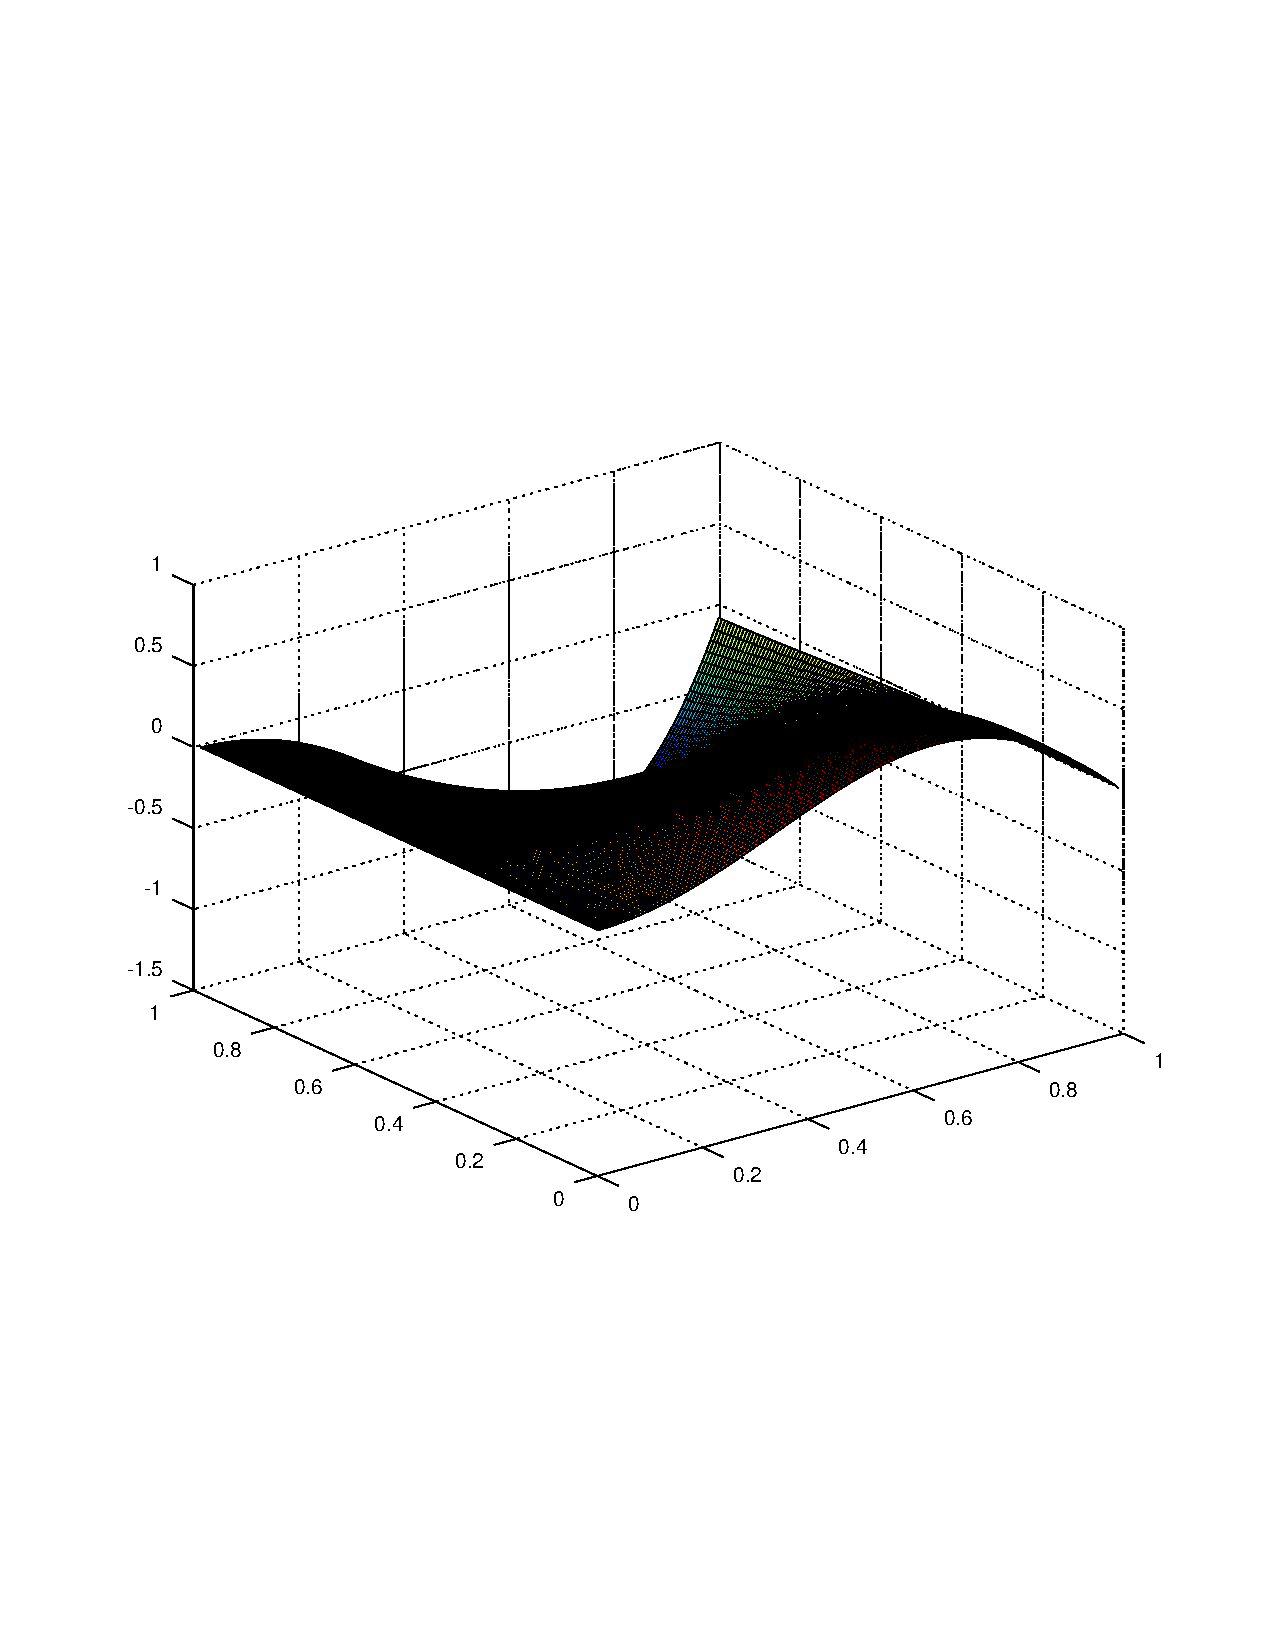
\includegraphics[scale=0.5]{malha128eg}

Cujo gráfico também aproxima-se do resultado esperado.

\section{Conclusão}

Os experimentos numéricos foram fundamentais para que conclusões e comparações entre as implementações fossem obtidas.

É possível notar a maior rapidez de resolução do sistema linear com uso do algoritmo de Gauss através da implementação em MatLab. A implementação built-in e tratada em baixo nível por essa linguagem para solução exata de sistemas lineares viabilizam que este processo seja mais rápido na ordem de milhares ao comparar com a abordagem utilizada na linguagem C.

Por outro lado, o SOR viu-se prejudicado no MatLab, agora sem comando built-in a ser utilizado como no Gauss. Os testes realizados na implementação em C demonstraram maior agilidade na hora da resolução por SOR.

Portanto, para que seja escolhida a melhor forma de obter a solução de um problema de valor de contorno bidimensional como os aqui abordados, é necessário atentar aos algoritmos de resolução de sistemas lineares empregados e suas implementações entre as duas linguagens. É importante também considerar, ao fazer essa escolha, o grau de confiança e precisão desejada no resultado.

% ----------------------------------------------------------
% ELEMENTOS PÓS-TEXTUAIS
% ----------------------------------------------------------
\postextual

% ---
% Título e resumo em língua estrangeira
% ---

% \twocolumn[    		% INICIO DE ARTIGO EM DUAS COLUNAS

% titulo em inglês
\titulo{Solution of two dimensional boundary conditions problems}
\emptythanks
\maketitle

% resumo em português
\renewcommand{\resumoname}{Abstract}
\begin{resumoumacoluna}
 \begin{otherlanguage*}{english}
   This essay describes the program implementation that solves two dimensional boundary conditions problems with also Gauss elimination and SOR algorithms, that were made in C and MatLab programming languages, using sparse matrix storage techniques, during the discretization through the finite difference method.

   \vspace{\onelineskip}
 
   \noindent
   \textbf{Keywords}: diferential equations. linear systems. boundary conditions. finite difference. discretization.
 \end{otherlanguage*}  
\end{resumoumacoluna}

% ]  				% FIM DE ARTIGO EM DUAS COLUNAS
% ---

% ----------------------------------------------------------
% Referências bibliográficas
% ----------------------------------------------------------
\bibliography{abntex2-modelo-references}

% ----------------------------------------------------------
% Glossário
% ----------------------------------------------------------
%
% Há diversas soluções prontas para glossário em LaTeX. 
% Consulte o manual do abnTeX2 para obter sugestões.
%
%\glossary

% ----------------------------------------------------------
% Apêndices
% ----------------------------------------------------------

% ---
% Inicia os apêndices
% ---

% ---

% ----------------------------------------------------------
% Anexos
% ----------------------------------------------------------
\cftinserthook{toc}{AAA}
% ---
% Inicia os anexos
% ---
%\anexos


\end{document}
